\documentclass[10pt]{article}

\usepackage{adjustbox}
\usepackage{amsmath}
\usepackage[french, onelanguage]{algorithm2e}
\usepackage[utf8]{inputenc}
\usepackage[french]{babel}
\usepackage{csquotes}
\usepackage[T1]{fontenc}
\usepackage{geometry}
\usepackage{glossaries}
\usepackage{graphicx}
\usepackage[hidelinks]{hyperref}
\usepackage[utf8]{inputenc}
\usepackage{listings}
\usepackage{lstautogobble}
\usepackage{tabularx}
\usepackage{textcase}
\usepackage{tikz}
\usepackage{tocloft}
\usepackage{verbatim}
\usepackage{xcolor}
%\usepackage[pdf]{pstricks}
%\usepackage{auto-pst-pdf}
%\usepackage{uml}

\makeglossaries

\newacronym{gui}{GUI}{Graphical User Interface}
\newacronym{jdk}{JDK}{Java Development Kit}
\newacronym{ram}{RAM}{Random Access Memory}
\newacronym{json}{JSON}{JavaScript Oriented Notion}
\newacronym{ttmc}{TTMC}{Tu te mets combien?}
\newacronym{po}{PO}{Product Owner}

\usetikzlibrary{calc, shapes.multipart, chains, arrows}

\definecolor{RoyalBlue}{cmyk}{1, 0.50, 0, 0}

\lstset{language=Java,
  keywordstyle=\color{RoyalBlue},
  basicstyle=\scriptsize\ttfamily,
  commentstyle=\ttfamily\itshape\color{darkgray},
  stringstyle=\ttfamily,
  breaklines=true,
  keepspaces=true,
  numbers=left,
  numbersep=5pt,
  showspaces=false,
  showstringspaces=false,
  showtabs=false,
  tabsize=4,
  autogobble=true
}

\geometry{
  a4paper,
  total={170mm,257mm},
  left=20mm,
  top=20mm,
}

\title{What do you know about it?}
\author{Giorgio Caculli LA196672, Guillaume Lambert LA198116, Tanguy Taminiau LA199566 \\ Groupe B05}
\date{\today}

\begin{document}
\maketitle

\newpage
\tableofcontents

\newpage
\section*{Introduction}
\label{sec:intro}
\addcontentsline{toc}{section}{\nameref{sec:intro}}
Dans le cadre du cours de ``Projets'' de l'UE 210, nous allons devoir créer un jeu similaire à ``\acrlong{ttmc}'' (\acrshort{ttmc}). L'objectif pédagogique de ce projet est de pousser l'élève a mieux appréhendé la librairie JavaFX vu au cours de 
POO (programmation orienté object). De plus la grande liberté accordé à ce projet consent et oblige l'élève à apprendre à se documenter et savoir faire des recherches.  L'objectif du projet est simple, créer un jeu sur le principe de TTMC (Tu Te 
mets Combien ?).  

\begin{comment}
\newpage
\section{Analyse de l'existant}
\subsection{Product backlog}
\noindent\adjustbox{max width=\textwidth}{
\begin{tabular}{| p{1cm} | p{16cm} |}
	\hline
	US-01 & En tant qu'utilisateur je voudrais savoir mon score.\\
	\hline
	US-02 & En tant qu'utilisateur je voudrais savoir si j'ai bien répondu.\\
	\hline
	US-03 & En tant qu'utilisateur je voudrais savoir si j'ai mal répondu.\\
	\hline
	US-04 & En tant qu'utilisateur je voudrais savoir quelle était la bonne réponse.\\
	\hline
	US-05 & En tant qu'utilisateur je voudrais savoir mettre mon jeu sur pause.\\
	\hline
	US-06 & En tant qu'utilisateur je voudrais savoir reprendre mon jeu où je l'avait laissé.\\
	\hline
	US-07 & En tant qu'utilisateur je voudrais savoir arrêter mon jeu à tout moment.\\
	\hline
	US-08 & En tant qu'utilisateur j'aimerais joué en multi joueur localement.\\
	\hline
	US-09 & En tant qu'administrateur je dois pouvoir ajouter une nouvelle carte au deck.\\
	\hline
	US-10 & En tant qu'administrateur je veux pouvoir supprimer une carte du deck.\\
	\hline
	US-11 & En tant qu'administrateur je veux pouvoir modifier une carte existante.\\
	\hline
	US-12 & En tant qu'utilisateur j'aimerais avoir une musique de fond.\\
	\hline
	US-13 & En tant qu'utilisateur j'aimerais pouvoir gérer le volume de la musique.\\
	\hline
	US-14 & En tant qu'utilisateur j'aimerais pouvoirs activer ou désactiver la musique de fond.\\
	\hline
	US-15 & En tant qu'utilisateur je voudrais pouvoir choisir mon propre pseudonyme.\\
	\hline
	US-16 & En tant qu'utilisateur je voudrais voir un plateau de jeu.\\
	\hline
	US-17 & En tant qu'utilisateur je voudrais avoir mon pion.\\
	\hline
	US-18 & En tant qu'utilisateur je voudrais savoir reconnaitre mon pion.\\
	\hline
	US-19 & En tant que joueur, je voudrais communiquer avec d'autre joueurs.\\
	\hline
	US-20 & En tant que joueur, j'aimerais jouer avec d'autre joueurs en ligne.\\
	\hline
	US-21 & En tant que joueur, j'aimerais rejoindre une partie en ligne.\\
	\hline
	US-22 & En tant que joueur, j'aimerais héberger une partie en ligne.\\
	\hline
\end{tabular}
}

\subsection{Les classes}

\subsubsection{Le modèle}

\subsubsection{La vue}

\subsubsection{Les exceptions}

\section{Description général de l'application}
Voici l'histoire d'un nain capable de courir vite et de voyager loin.\\
Dans son épopée formidable nous le suivrons une bière à la main.\\

\end{comment}

\newpage
\section{Product backlog}
\noindent\adjustbox{max width=\textwidth}{
\begin{tabular}{| p{1cm} | p{16cm} |}
	\hline
	US-01 & En tant qu'utilisateur je voudrais savoir mon score.\\
	\hline
	US-02 & En tant qu'utilisateur je voudrais savoir si j'ai bien répondu.\\
	\hline
	US-03 & En tant qu'utilisateur je voudrais savoir si j'ai mal répondu.\\
	\hline
	US-04 & En tant qu'utilisateur je voudrais savoir quelle était la bonne réponse.\\
	\hline
	US-05 & En tant qu'utilisateur je voudrais savoir mettre mon jeu sur pause.\\
	\hline
	US-06 & En tant qu'utilisateur je voudrais savoir reprendre mon jeu où je l'avait laissé.\\
	\hline
	US-07 & En tant qu'utilisateur je voudrais savoir arrêter mon jeu à tout moment.\\
	\hline
	US-08 & En tant qu'utilisateur j'aimerais joué en multi joueur localement.\\
	\hline
	US-09 & En tant qu'administrateur je dois pouvoir ajouter une nouvelle carte au deck.\\
	\hline
	US-10 & En tant qu'administrateur je veux pouvoir supprimer une carte du deck.\\
	\hline
	US-11 & En tant qu'administrateur je veux pouvoir modifier une carte existante.\\
	\hline
	US-12 & En tant qu'utilisateur j'aimerais avoir une musique de fond.\\
	\hline
	US-13 & En tant qu'utilisateur j'aimerais pouvoir gérer le volume de la musique.\\
	\hline
	US-14 & En tant qu'utilisateur j'aimerais pouvoirs activer ou désactiver la musique de fond.\\
	\hline
	US-15 & En tant qu'utilisateur je voudrais pouvoir choisir mon propre pséudonyme.\\
	\hline
	US-16 & Création d'un plateau de jeu.\\
	\hline
	US-17 & Implémentation du plateau de jeu.\\
	\hline
	US-18 & Creation des pions.\\
	\hline
	US-19 & Implémentation des pions de jeu et animation de mouvements des pions.\\
	\hline
	US-20 & Investiguer sur le multi joueur en ligne.\\
	\hline
	US-21 & Pion personnaliser.\\
	\hline
	US-22 & En tant que joueur, je voudrais communiquer avec d'autre joueur.\\
	\hline
	US-23 & En tant que joueur, j'aimerais jouer avec d'autre joueur en ligne.\\
	\hline
	US-24 & En tant que joueur, j'aimerais rejoindre une partie en ligne.\\
	\hline
	US-25 & En tant que joueur, j'aimerais héberger une partie en ligne.\\
	\hline
\end{tabular}
}


\newpage
\section{Tableau Trello}
\begin{figure}[ht]
	\centering
	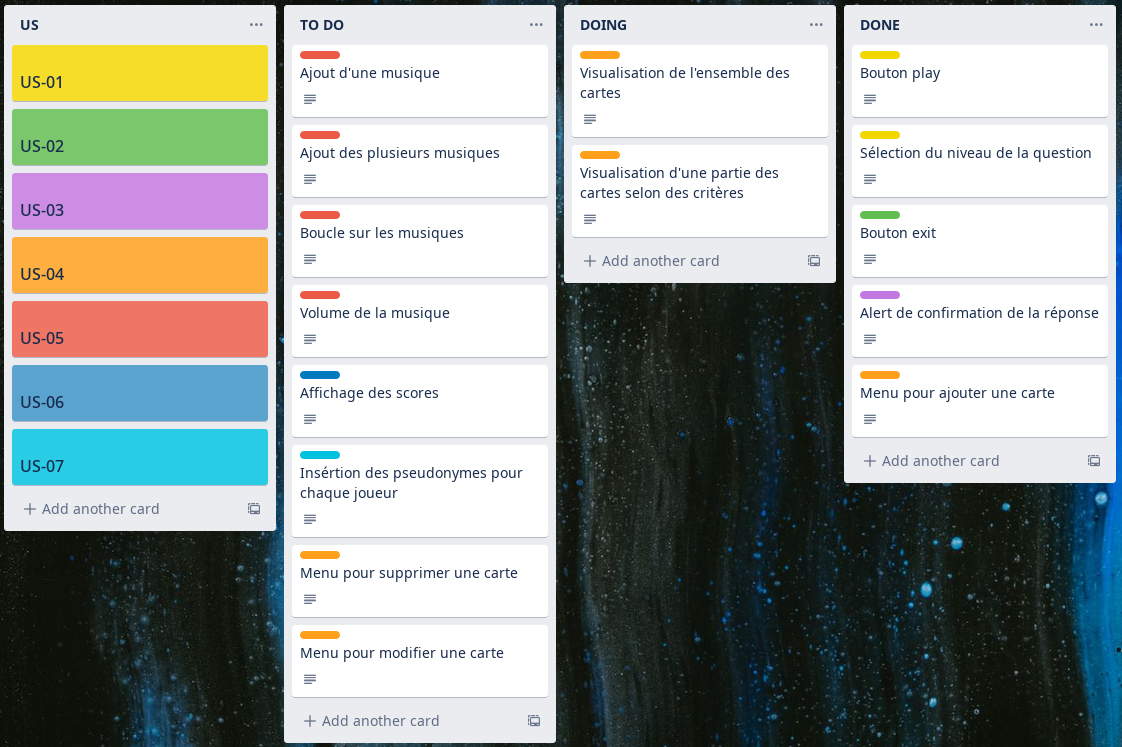
\includegraphics[width=\textwidth]{trello_1.png}
	\caption{Tableau Trello Sprint 1}
	\label{Tableau Trello Sprint 1}
\end{figure}


\newpage
\section{Diagramme de classe}
%\umlDiagram[box=,sizeX=7cm, sizeY=7cm]{
%	\umlClass[]{Deck}
%	{}
%	{
%		\umlMethod[visibility]{add}{c \emph{BasicCard}}
%		\umlMethod[visibility]{remove}{c \emph{BasicCard}}
%		\umlMethod[visibility]{remove}{i \emph{int}}
%	}
%}
\begin{figure}[h]
	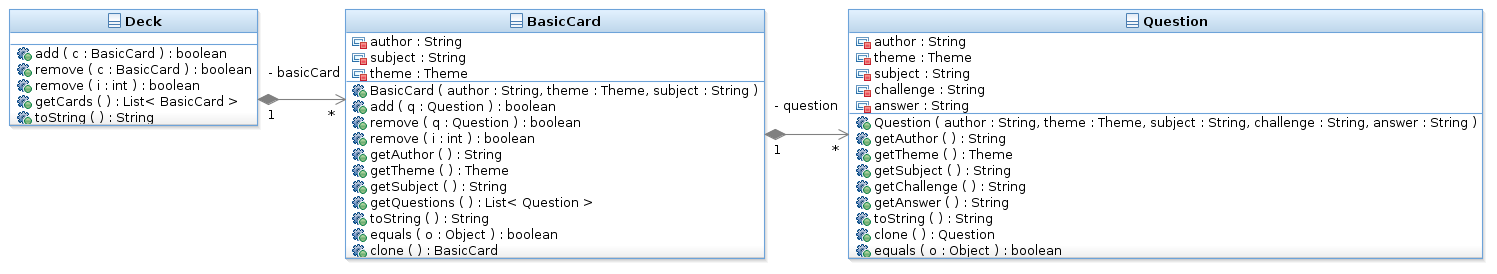
\includegraphics[width=\textwidth]{TTMC_Model_Diagram.png}
	\centering
\end{figure}

\begin{comment}
\newpage
\section{Plan de sortie}
\begin{figure}[h]
	\centering
	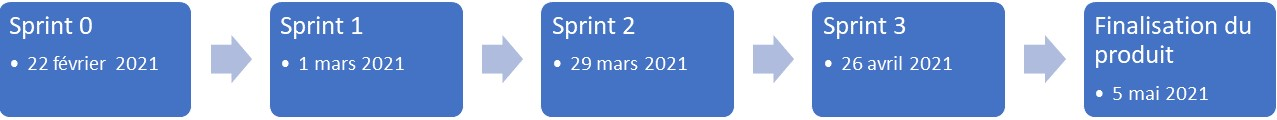
\includegraphics[width=\textwidth]{plan.jpg}
	\caption{Release plan}
	\label{fig:plan}
\end{figure}
\begin{itemize}
	\item Sprint 0 - Analyse et recherche.\\
	Cette première étape nous permettra de mettre en place le modèle du projet sur base de ce qui a été trouvé sur internet. Une fois compris les règles, il sera possible d'établir les fonctionnalités de base pour les composants principaux du programme ainsi que la mise en place des règles qui caractérisent chaque composant.
	\item Sprint 1 - Première démonstration en présence du Product Owner.\\
	Lors de la première démonstration, les différentes fonctionnalités seront testées. Les tests unitaires ne renverront aucun erreur et les différentes exceptions qui caractérisent chaque composant seront gérées.
	\item Sprint 2 - Deuxième démonstration du produit.\\
	Lors de la deuxième démonstration, un programme avec interface interactive sera mis en place. Ce prototype permettra d'interagir avec les différentes composantes et les manipuler librement.
	\item Sprint 3 - Troisième et dernière démonstration.\\
	Lors de la troisième démonstration, le programme aura une interface graphique basée sur JavaFX et toutes les interactions seront finalisées.
	\item Finalisation du produit - Présentation du produit final au client.\\
	Tous les bugs seront corrigés et toutes les interactions prévues seront fonctionnelles.
\end{itemize}

\newpage
\section{Prototype}
Dans cette section, nous vous présentons le prototype graphique.

\subsection{Menu principal}
Voici le menu principal, depuis celui-ci, il sera possible de jouer, de paramétrer le jeu, de quitter le jeu ou alors de gérer le jeu.
\begin{figure}[ht]
	\centering
	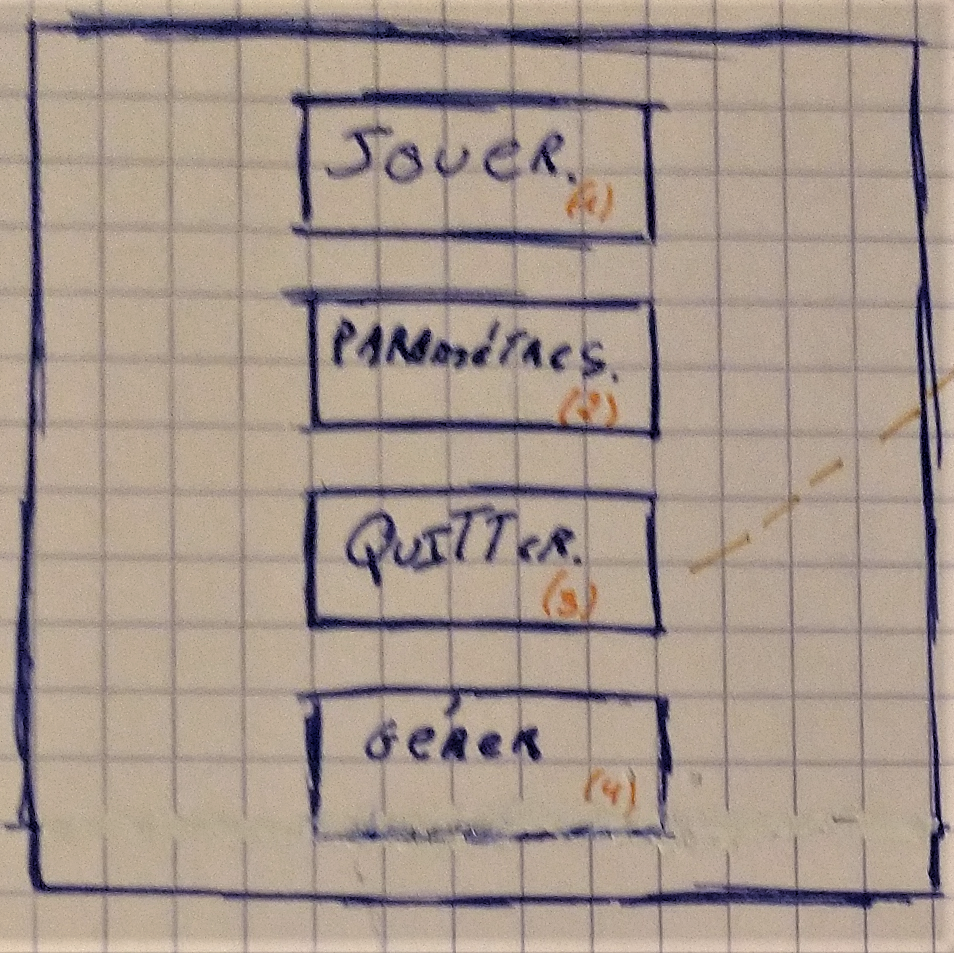
\includegraphics[scale=0.5]{menu_principal.png}
	\caption{menu principal}
	\label{interface menu}
\end{figure}

\newpage
\subsection{Menu joueur}
Le menu joueur sera un combo de label et de textfield, il sert à prendre des informations sur le nom des équipes. Il faut au minimum deux équipes ou joueurs.
\begin{figure}[ht]
	\centering
	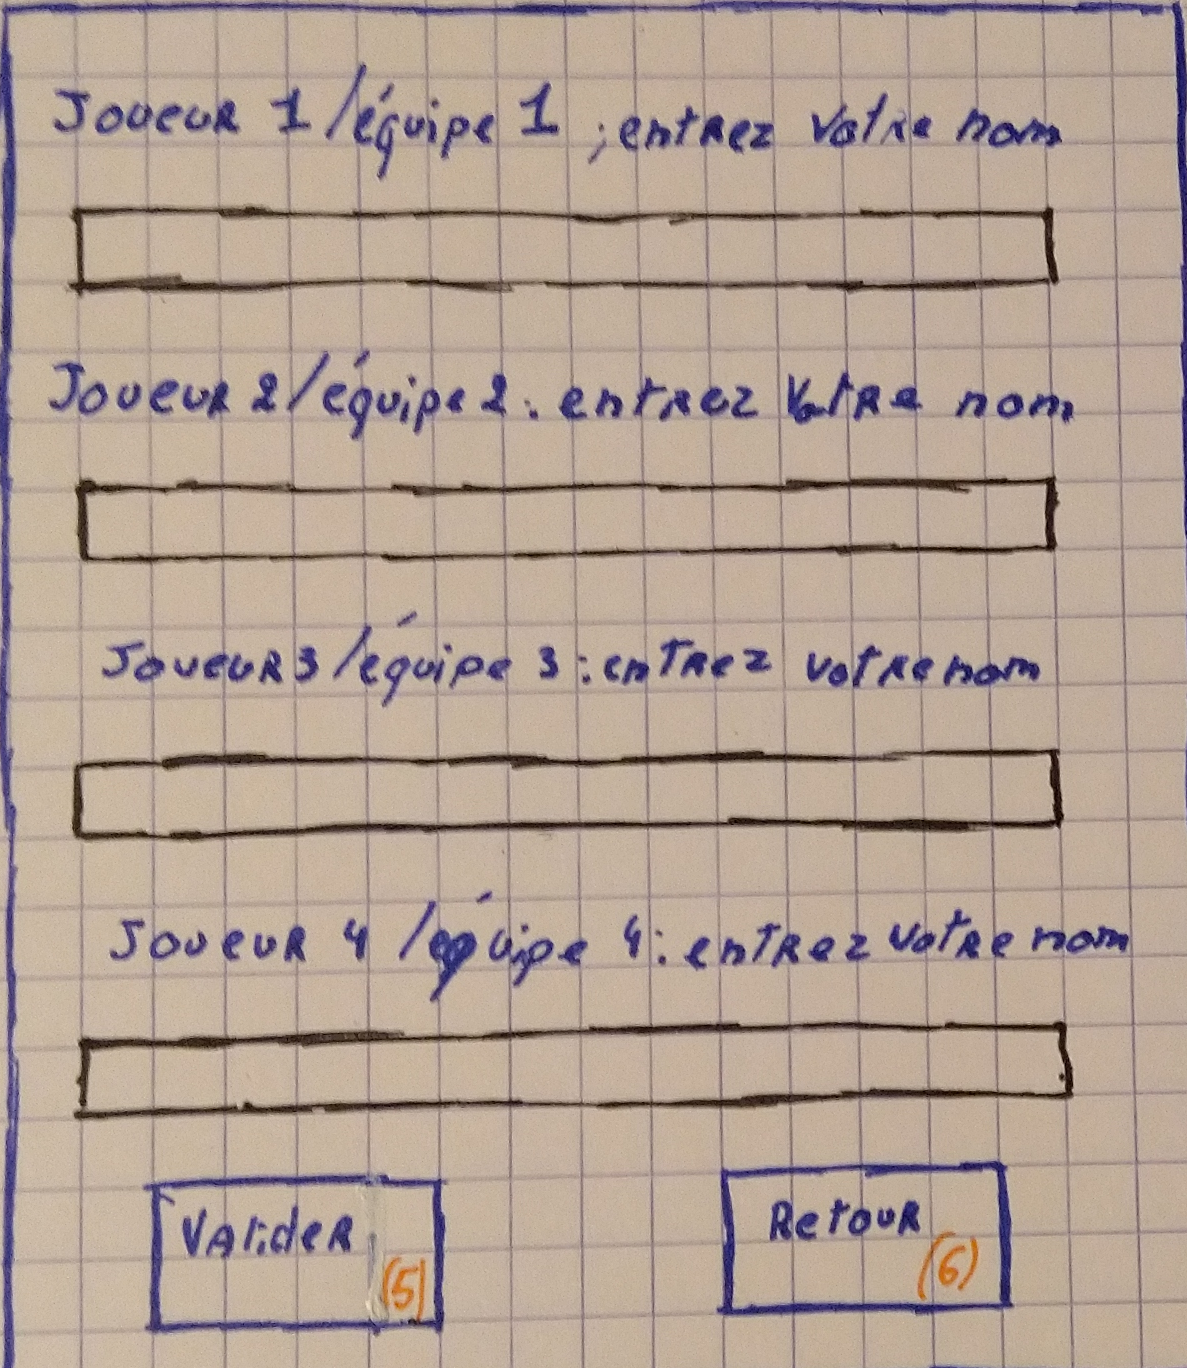
\includegraphics[scale=0.5]{menu_joueur.png}
	\caption{nom des joueurs ou équipe}
	\label{interface création d'équipe}
\end{figure} 

\newpage
\subsection{Fênetre erreur du nombre de joueurs}
Dans le cas où l'on n'entre pas suffisamment de joueur ou d'équipe, une alerte va notifier le joueur qu'il n'y a pas assez de joueur et ne peut donc pas jouer dans que cela n'est pas réglé.
\begin{figure}[ht]
	\centering
	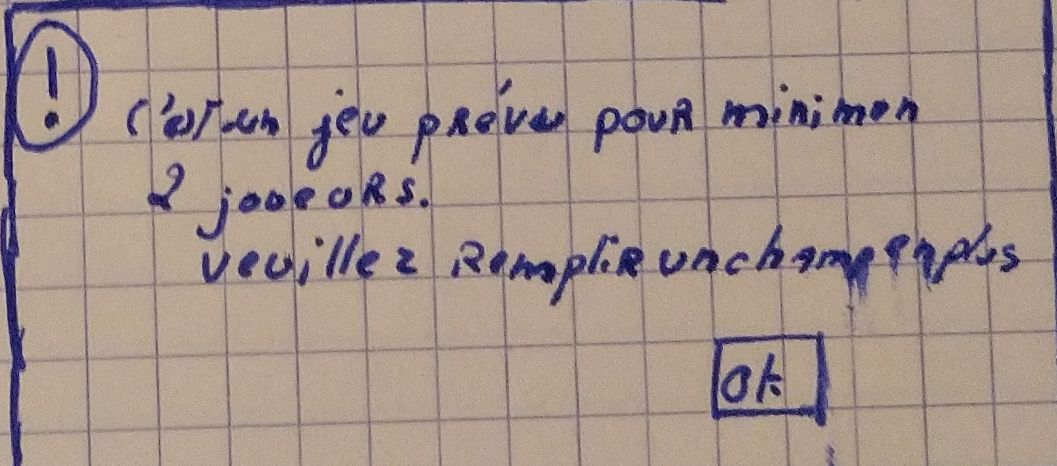
\includegraphics[scale=0.5]{fenetre_erreur_nb_joueur.png}
	\caption{alerte de non conformité du nombre de joueurs}
	\label{alerte du nombre de joueurs}
\end{figure}

\newpage
\subsection{Jeu}
Le UI sera composé d'un label avec le nom de l'équipe, un autre avec un des quatre thèmes, et un dernier avec le sujet de la question. Ensuite, il y a quatre boutons cliquable avec un numéro de un à quatre. Le numéro sur le bouton correspond 
à la difficulté de la question par ordre croissant.
\begin{figure}[ht]
	\centering
	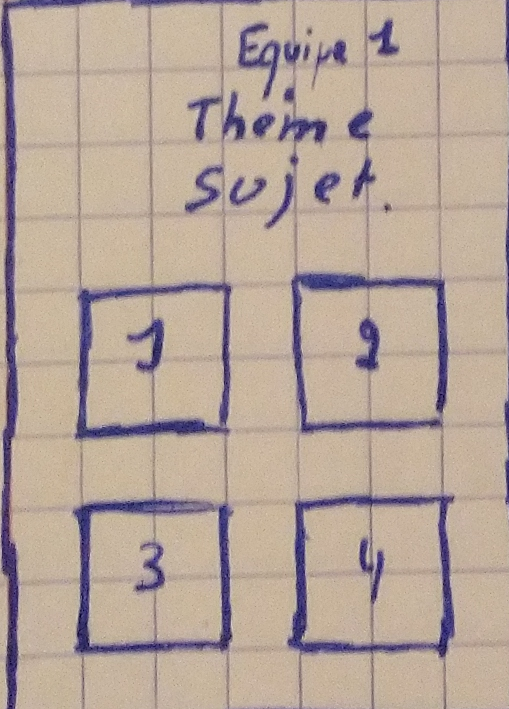
\includegraphics[scale=0.5]{jeux.png}
	\caption{choix de la difficulté de la question}
	\label{interface jeu}
\end{figure}

\newpage
\subsection{Fênetre quitter}
Il s'agit d'une fênetre permettant de vérifier si le joueur veux réellement quitter la partie. Cette fênetre est composer d'un label et de deux boutons permettant soit de quitter l'application, soit de retourner au menu principal.
\begin{figure}[ht]
	\centering
	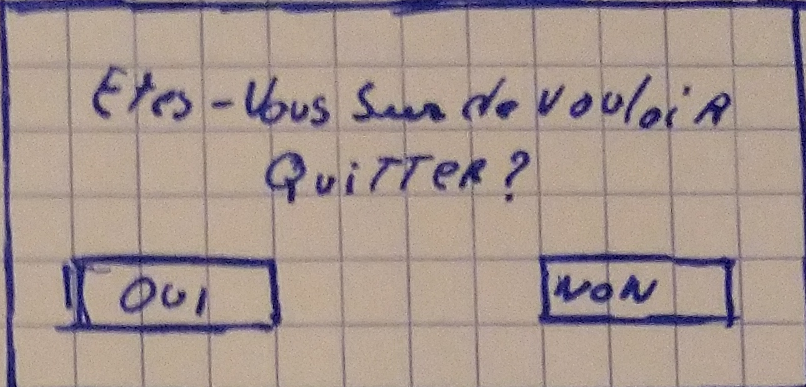
\includegraphics[scale=0.5]{fenetre_quitter.png}
	\caption{fêntre pour quitter le jeu}
	\label{fênetre pour quitter le jeu}
\end{figure} 

\end{comment}

\newpage
\section{Code le plus représentatif}
Code les plus représentatifs du Sprint 1
\begin{lstlisting}
  public void setVisibleNode( String paneName )
  {

    for ( Node n : getStackPane().getChildren() )
    {
      if ( n.getClass().getSimpleName().equals( paneName ) )
      {
        n.setVisible( true );
      }
      else
      {
        n.setVisible( false );
      }
    }
  }
  

  getStackPane().getChildren().add( new MenuPrincipalBP( d ) );
  getStackPane().getChildren().add( new MenuPlayBP( d ) );
  getStackPane().getChildren().add( new MenuAdminBP( d ) );

  setVisibleNode( MenuPrincipalBP.class.getSimpleName() );
\end{lstlisting}

Ce code permet de choisir quel Node le stackpane devrait rendre visible sur base d'une chaîne de caractère.
Tous les autres Node seront cachés si le nom de la classe ne corréspond pas à celle qu'on souhaite visible.
Indépendammente de l'ordre, la fonction sera capabe de rendre un seul Pane visible.

Ici par exemple, une StackPane contient 3 Node:
\begin{itemize}
\item MenuPrincipalBP
\item MenuPlayBP
\item MenuAdminBP
\end{itemize}

Lors de l'appel de la fonction setVisibleNode, on prendra en paramètre une chaîne de caractère, soit le nom de la classe que l'on souhaite charger.

On peut obtenir le nom de la classe sans faire aucune faute de frappe, en appelant fonction propre à chaque classe: \verb|getSimpleName()|.
Grâce à cette fonction, peut importe la casse, le paneName introduit sera toujours celui du Node qu'on souhaite montrer.


\newpage
\section{Sprint review}
Durant ce deuxième sprint,\\
Nous avons créé de nouvelles interactions entre l'utilisateur et le logiciel de jeu.
Nous avons développé une interface pour afficher les cartes.
Une nouvelle fonctionnalité concernant la gestion des cartes a également été programmée, il s'agit de la possibilité de supprimer une carte du deck.
Autre changement concernant la gestion des cartes, l'interface permettant de modifier les cartes est également opérationnelle.
Les options présentées ci-dessus sont accéssible depuis le menu administrateur.
Le jeu lui-même a également bénéficié d'ajout tel qu'un système de score.
Un multi joueur local a aussi été créé (pour le moment uniquement en 1v1).
Le jeu prend en charge les pseudos pour une partie multi joueur locale tout comme pour une partie solo.
Un menu pause a également été créé, celui-ci permet de mettre en pause la partie.
Depuis ce menu, il est possible soit de reprendre la partie ou de la quitter.
Des animations et un timer ont été rajoutés afin de rendre le jeu plus intéressant et dynamique.
Afin de rendre le jeu agréable nous avons ajouté une playlist de musiques ainsi que quelques fonctionnalités pour pouvoir gérer celle-ci.
Dernière modification concernant le jeu, l'interface de jeu prend comme couleur de fond la couleur du thème de la carte tirée (c'est à dire, lors du choix de la difficulté de la question ou lors d'y répondre, la couleur de fond de l'interface est colorée en rapport avec le thème la carte tirée).
Des interactions clavier-logiciel ont été créées, il est dès lors possible de, notamment, faire apparaitre le menu pause grace à la touche ESCAPE ainsi que d'utiliser la touche ENTER pour valider un choix.
Pour améliorer la sécurité du jeu, la fenêtre de login a été mise en place.
Nous avons décidé de créer un launcher pour notre jeu permettant aux utilisateurs n'ayant pas JavaFX de pouvoir quand même y jouer.\\
Une partie du travail fait durant ce sprint a également été de modifier quelques parties du code afin de satisfaire le \acrshort{po}.
Nous avons fait une conversion totale du code afin d'éviter d'utiliser plusieurs Scenes, la nouvelle solution mise en place est l'utilisation d'une seule et unique Scene, combinée à plusieurs StackPanes.  


\section{Sprint retrospective}
De manière générale, l'ensemble du groupe est toujours motivé et disponible pour parler et coder les différentes améliorations du programme.
En ce qui concerne le sprint qui vient de s'achever (Sprint 2), l'équipe complète est contente des résultats.
En effet, une partie assez conséquante du travail mené demandait beaucoup de temps et de recherche afin de pouvoir être incorporée dans le jeu.
Par exemple, la musique qui nous a demandé de faire des recherches sur le fonctionnement des Threads.
Le travail de débogage est également assez chronophage mais nous essayons toujours de traquer et traiter le plus de bugs possible, bien que nous en découvrions parfois encore.
Nous sommes contents du travail réalisé jusqu'à présent aussi bien dans son développement que dans la recherche des bugs, mais nous essayons toujours de découvrir des nouvelles technologies et de l'améliorer.


\section{Design pattern}
Afin d'assurer un certain niveau de securité lors des manipulations avec les cartes du deck, on a envisagé la possibilité de mettre en place un Proxy. Ceci, permettrai d'intéragir avec les carte à travers une interface qui aurait le seul et unique droit d'accéder à toutes les cartes présentes dans le Deck. Ce serait la seule qui aurait le droit d'écrire dans le deck.


\newpage
\printglossary

\end{document}
